\documentclass[letterpaper,12pt]{article}

%\usepackage{ucs}
%\usepackage[utf8x]{inputenc}
\usepackage{amsmath}
\usepackage{amsfonts}
\usepackage{amssymb}
\usepackage{graphicx}
%\usepackage[canadian]{babel}
\usepackage[margin=1in]{geometry}
\usepackage{multicol}
\newcommand{\R}{\mathbb{R}}
\renewcommand{\i}{\mathbf{i}}
\renewcommand{\j}{\mathbf{j}}
\renewcommand{\k}{\mathbf{k}}
\newcommand{\pd}[2]{\dfrac{\partial #1}{\partial #2}}
\newcommand{\di}{\displaystyle}

\title{Solutions to Quiz 11 Practice Problems\\Math 2580\\Spring 2016}
\author{Sean Fitzpatrick}
\date{February 25th, 2016}

\begin{document}
 \maketitle

\begin{enumerate}
 \item Evaluate the following iterated integrals:
\begin{enumerate}
 \item $\di \int_0^2\int_0^3x^2y^3\,dx\,dy=\int_0^2\left(\left.\frac{1}{3}x^3y^3\right|_0^3\right)\,dy = \int_0^2 9y^3\,dy = \left.\frac{9}{4}y^4\right|_0^2 = 36$.

 \item $\di \int_{-1}^1\int_0^2 x^2y\sin(y^2)\,dx\,dy = \int_0^2 x^2\left(\int_{-1}^1y\sin(y^2)\,dy\right)\,dx = 0$, since we're integrating a function that is odd (with respect to $y$) between symmetric limits.

 \item $\di \int_{-1}^1\int_0^3 y^5e^{xy^3}\,dx\,dy$

\medskip

Recall that when we perform the integral with respect to $x$ we're treating $y$ as a constant. We thus have
\[
 \int_0^3 y^5e^{xy^3}\,dx = \left.y^5\left(\frac{1}{y^3}e^{xy^3}\right)\right|_0^3 = y^2(e^{3y^3}-1).
\]
Putting this into the original integral gives us
\[
 \int_{-1}^1\int_0^3 y^5e^{xy^3}\,dx\,dy = \int_{-1}^1 (y^2e^{3y^3}-y^2)\,dy = \left.\frac{1}{9}e^{y^3}-\frac{1}{3}y^3\right|_{-1}^1 = \frac{e^3}{9}-\frac{e^{-3}}{9}-\frac{2}{3}.
\]

 \item $\di \int_0^\pi\int_{-\pi/2}^{\pi/2}\sin(x+y)\,dx\,dy$
\begin{align*}
 \int_0^\pi\int_{-\pi/2}^{\pi/2}\sin(x+y)\,dx\,dy & = \int_0^\pi\left(\left.-\cos(x+y)\right|_{x=-\pi/2}^{x=\pi/2}\right)\,dy\\
& = \int_0^\pi(-\cos(y+\pi/2)+\cos(y-\pi/2))\,dy\\
& = \left. -\sin(y+\pi/2)+\sin(y-\pi/2)\right|_0^\pi\\
& = -\sin(3\pi/2)+\sin(\pi/2)+\sin(\pi/2)-\sin(-\pi/2) = 4.
\end{align*}

\end{enumerate}
 \item Evaluate the following integrals over the given region $D$:
\begin{enumerate}
 \item $\di \iint_D x^3y^2\,dA$, where $D=\{(x,y) | 0\leq x\leq 2, -x\leq y\leq x\}$.

\medskip

Since the region is Type 1, we integrate first with resepct to $y$. Thus,
\begin{align*}
 \iint_D x^3y^2\,dA & = \int_0^2\int_{-x}^x x^3y^2\,dy\,dx\\
& = \int_0^2\left(\left.\frac{1}{3}x^3y^3\right|_{-x}^x\right)\,dx\\
& = \int_0^2 \frac{2}{3}x^6\,dx = \left.\frac{2}{21}x^7\right|_0^2\\
& = \frac{256}{21}.
\end{align*}


 \item $\di \iint_D (1-\sin(\pi x))\,dA$, where $D$ is the region bounded by the lines $y=x$, $y=0$, and $x=1$.

\medskip

The integral is of both Type 1 and Type 2, so we can integrate in either order. However, if we integrate first with respect to $y$, we'll be left with the integral of $x-x\sin(\pi x)$ with respect to $x$, requiring us to integrate by parts. We therefore integrate first with respect to $y$, giving us
\begin{align*}
 \iint_D (1-\sin(\pi x))\,dA & = \int_0^1\int_y^1(1-\sin(\pi x))\,dx\,dy\\
& = \int_0^1 \left(\left. x+\frac{1}{\pi}\cos (\pi x)\right|_y^1\right)\,dy\\
& = \int_0^1 \left(1-y-\frac{1}{\pi}-\frac{1}{\pi}\cos(\pi y)\right)\,dy\\
& = \left. \bigl(1-\frac{1}{\pi}\bigr)y-\frac{1}{2}y^2-\frac{1}{\pi^2}\sin(\pi y)\right|_0^1\\
& = \frac{1}{2}-\frac{1}{\pi}.
\end{align*}

\end{enumerate}
 \item For each of the iterated integrals below, (i) sketch the region of itegration, and (ii) evaluate the integral.
\begin{enumerate}
 \item $\di \int_0^\pi\int_{\sin x}^{3\sin x}x(1+y)\,dy\,dx$.

\bigskip

\begin{center}
 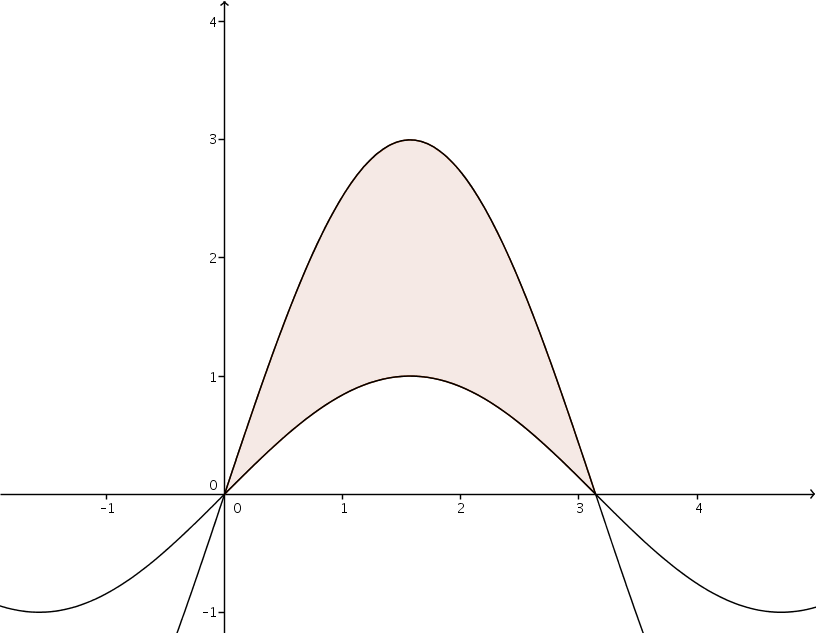
\includegraphics[width=3.5in]{Q11-3a.png}
\end{center}
We evaluate the iterated integral, using a trig identity and integration by parts to handle the integral with respect to $x$:
\begin{align*}
 \int_0^\pi\int_{\sin x}^{3\sin x}x(1+y)\,dy\,dx & = \int_0^\pi\left(x\left.\left(y+\frac{1}{2}y^2\right)\right|_{\sin x}^{3\sin x}\right)\,dx\\
& = \int_0^\pi x(2\sin x+4\sin^2 x)\,dx\\
& = \int_0^\pi x(2\sin x+2-2\cos(2x))\,dx\\
& = \left. -2x\cos x+2\sin x+x^2-x\sin(2x)+\frac{1}{2}\cos(2x)\right|_0^\pi\\
& = \pi^2+2\pi.
\end{align*}

 \item $\di \int_0^1\int_0^{x^2}(x^2+xy-y^2)\,dy\,dx$.

\begin{center}
 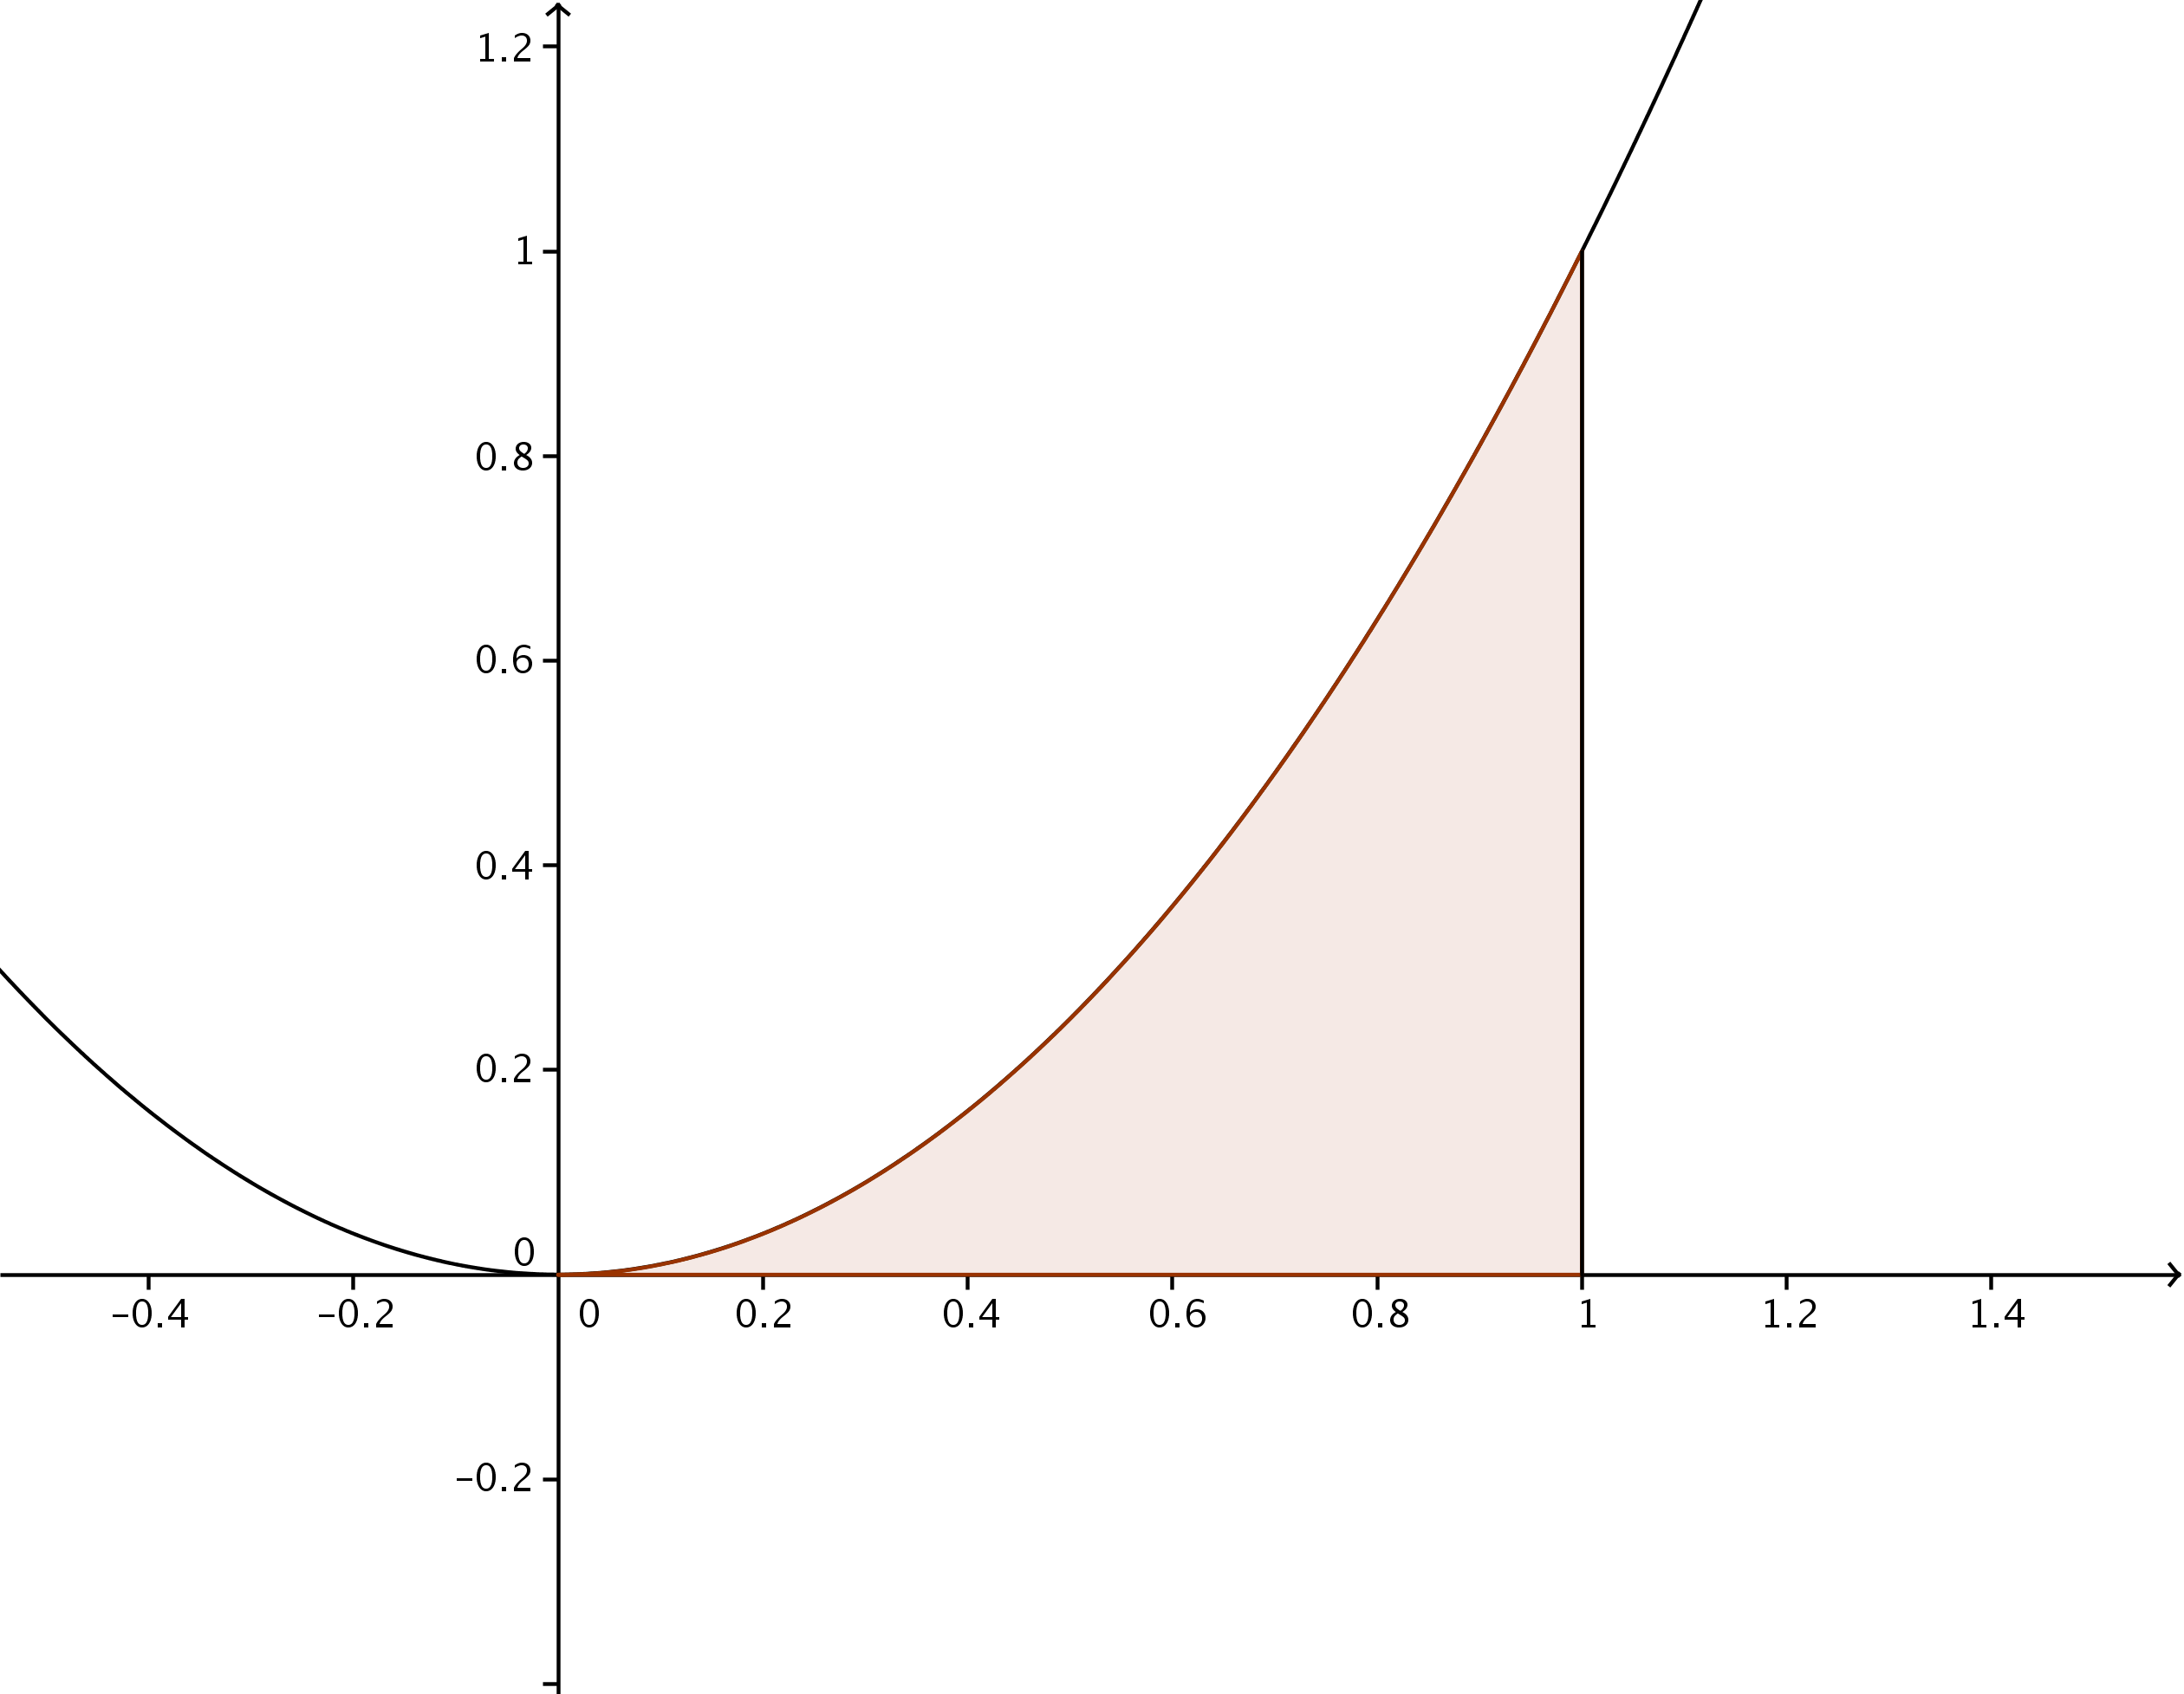
\includegraphics[width=3.5in]{Q11-3b.png}
\end{center}

\begin{align*}
 \int_0^1\int_0^{x^2}(x^2+xy-y^2)\,dy\,dx & = \int_0^1\left.\left(x^2y+\frac{1}{2}xy^2-\frac{1}{3}y^3\right)\right|_0^{x^2}\,dx\\
& = \int_0^1 \left(x^4+\frac{1}{2}{x^5}-\frac{1}{3}x^6\right)\,dx\\
& = \frac{1}{5}+\frac{1}{12}-\frac{1}{21} = \frac{33}{140}.
\end{align*}

\end{enumerate}
 \item For each of the iterated integrals below, (i) sketch the region of integration, (ii) change the order of integration, and (iii) evaluate the integral.

 \begin{enumerate}
  \item $\di \int_0^1\int_0^x xy\,dy\,dx$

\begin{center}
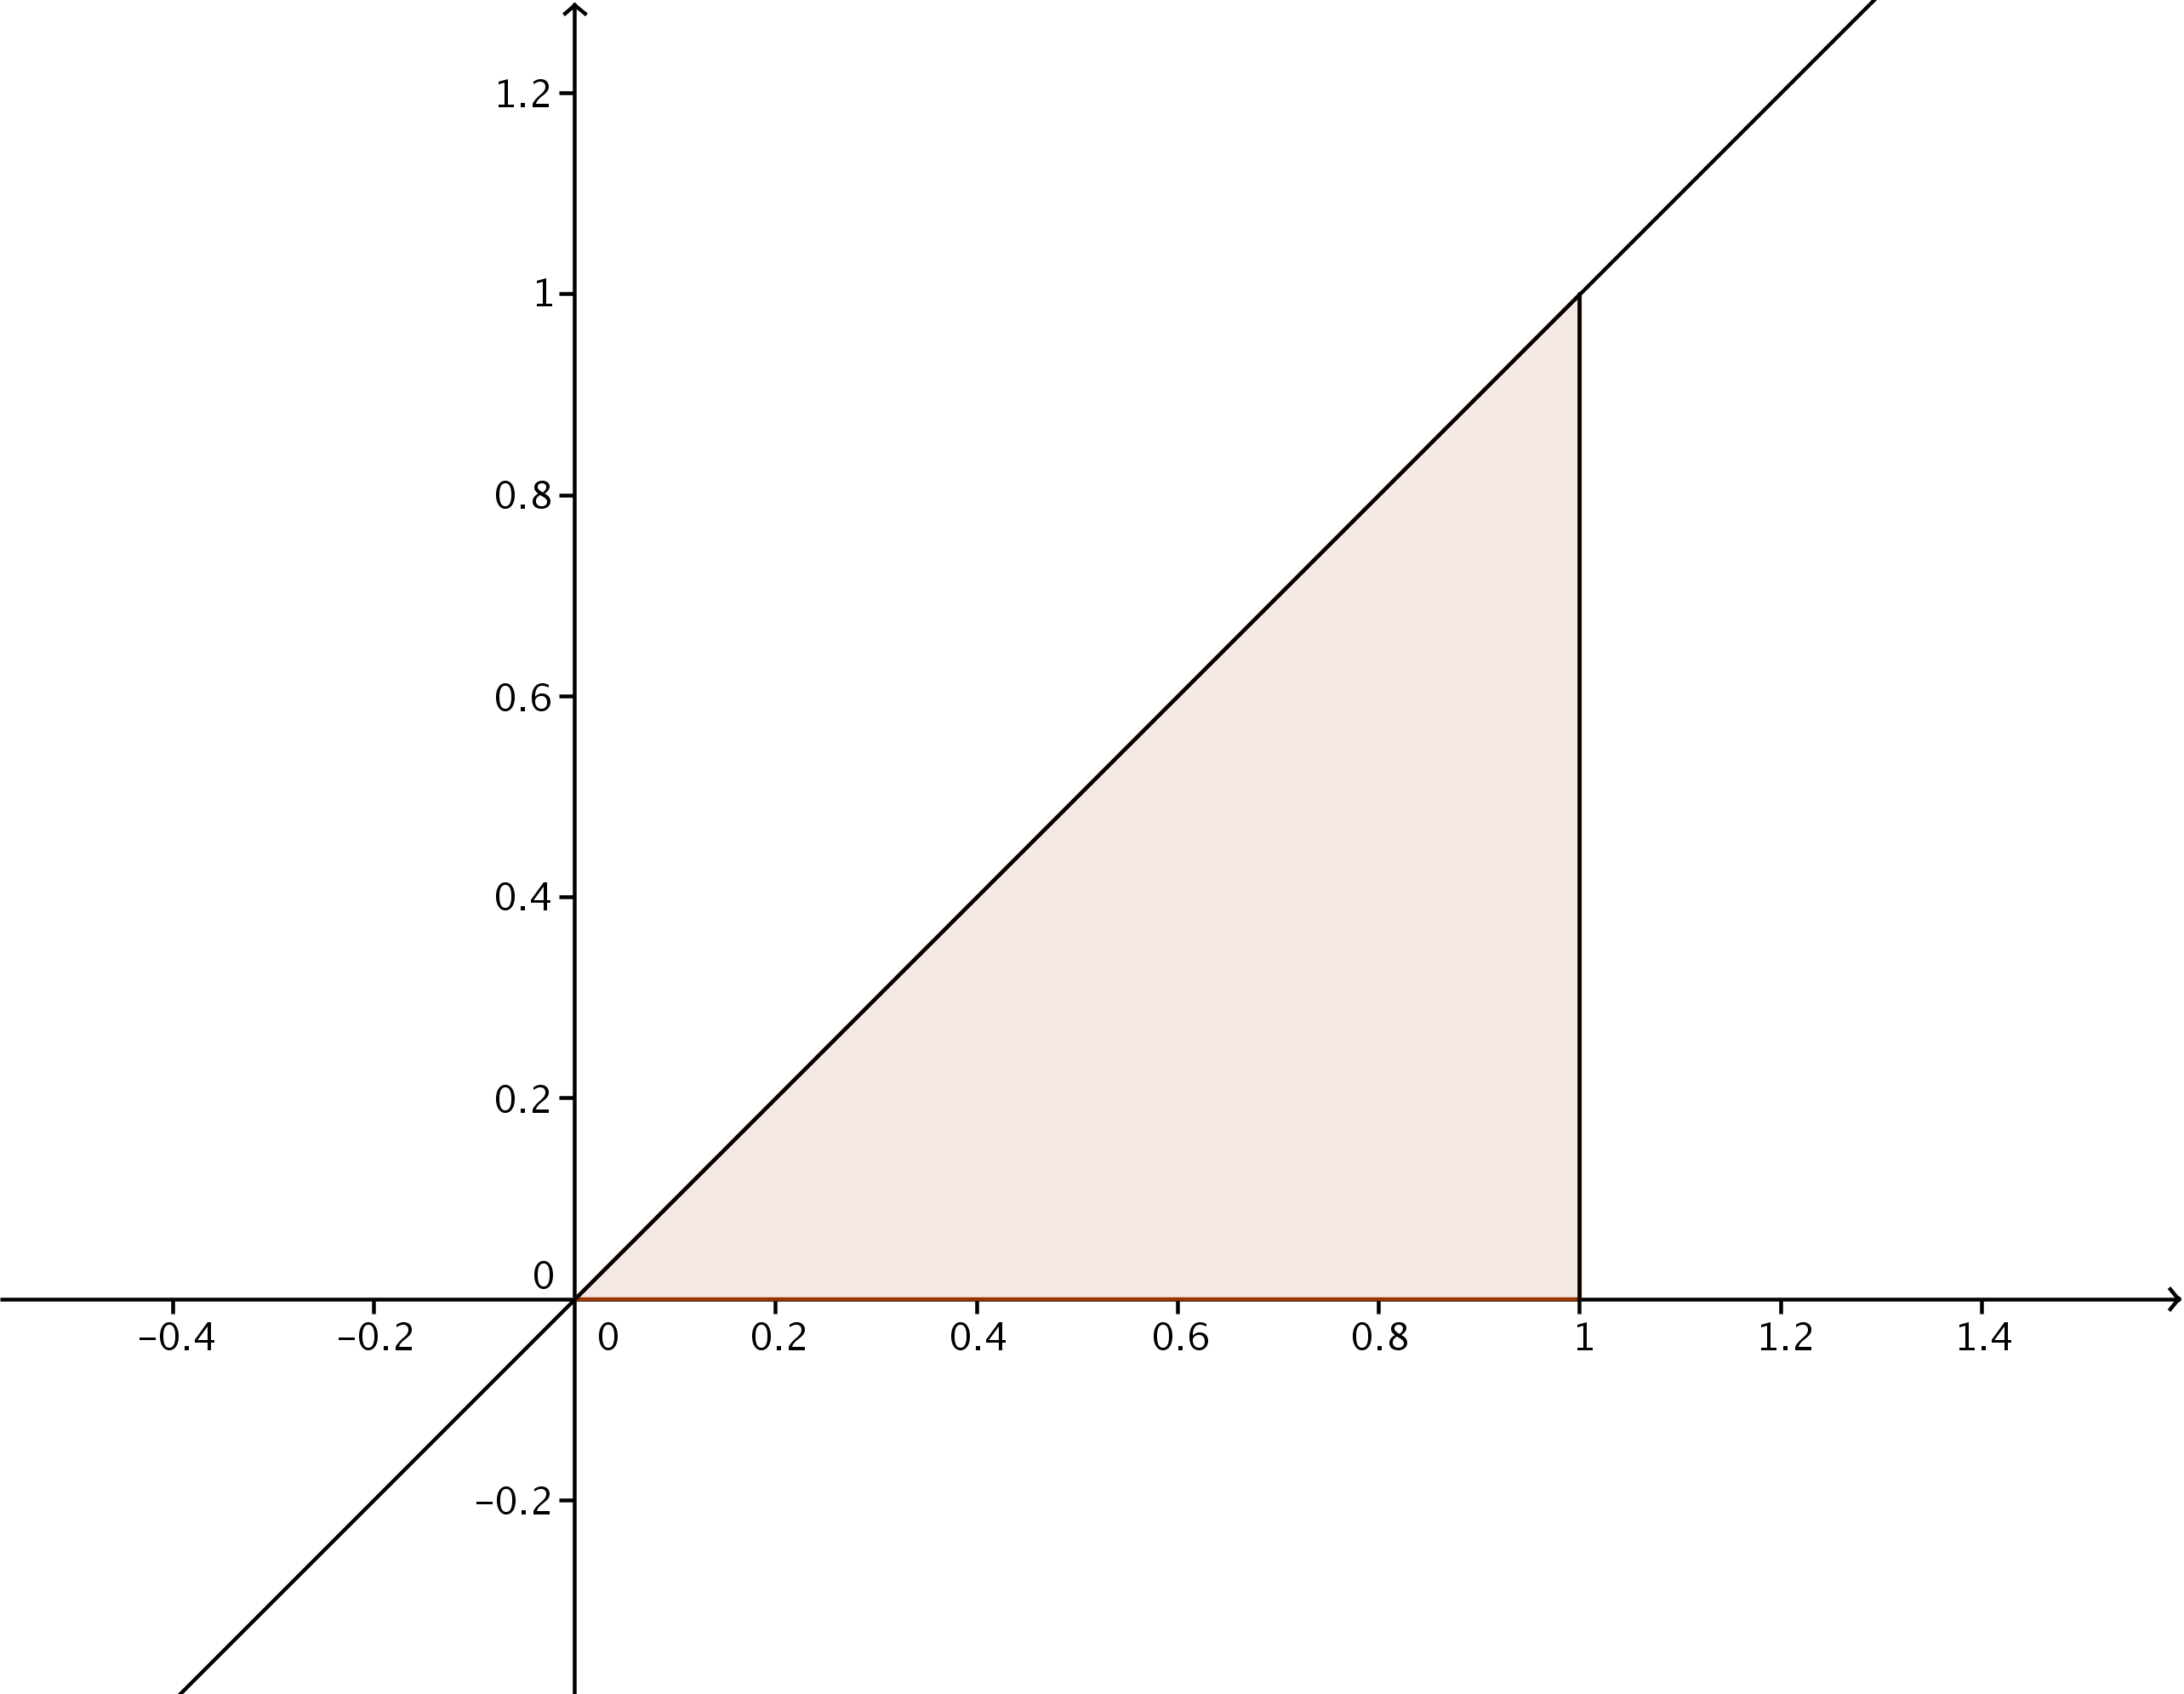
\includegraphics[width=3.5in]{Q11-4a.png} 
\end{center}

The region is given as the Type 1 region $0\leq x\leq 1$, $0\leq y\leq x$. We can express it as the Type 2 region $0\leq y\leq 1$, $y\leq x\leq 1$, giving us
\begin{align*}
 \int_0^1\int_0^x xy\,dy\,dx & = \int_0^1 \int_y^1 xy\,dx\,dy\\
& = \int_0^1\left(\left.\frac{1}{2}x^2y\right|_y^1\right)\,dy\\
& = \frac{1}{2}\int_0^1(y-y^3)\,dy\\
& = \frac{1}{2}\left(\frac{1}{2}-\frac{1}{4}\right) = \frac{1}{8}.
\end{align*}

  \item $\di \int_0^1\int_{1-y}^1(x+y^2)\,dx\,dy$

\begin{center}
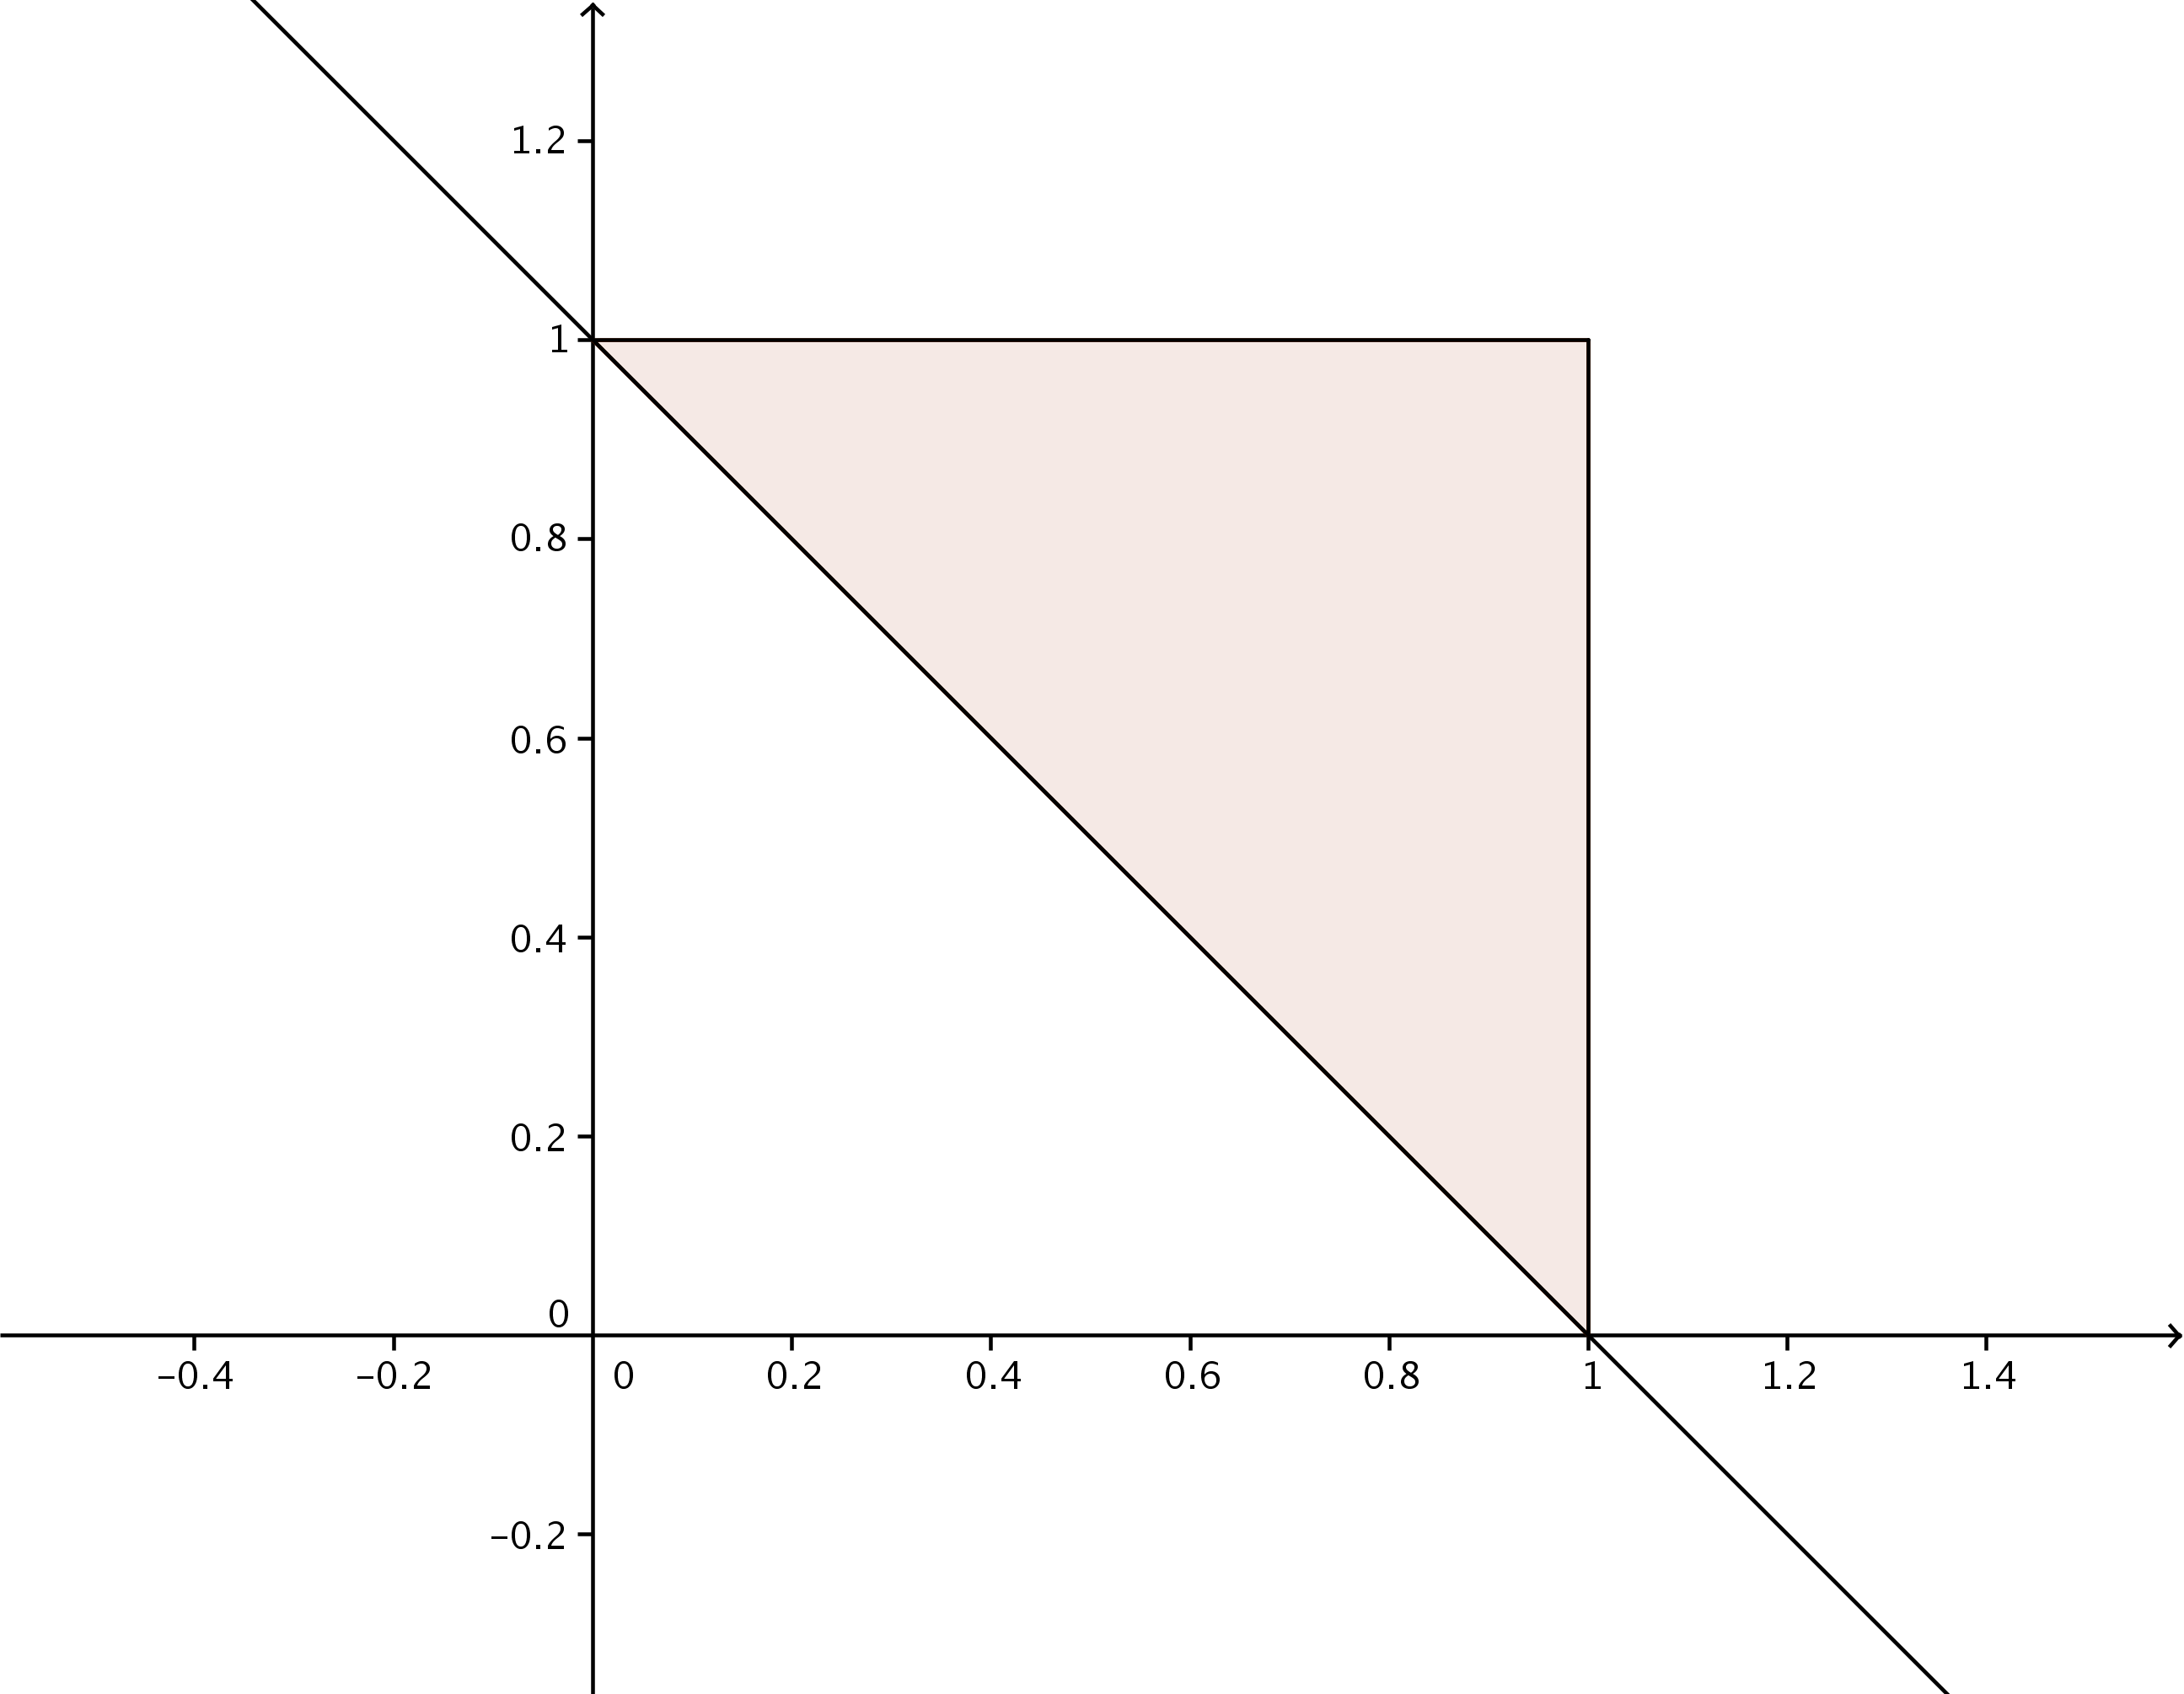
\includegraphics[width=3.5in]{Q11-4b.png} 
\end{center}

The Type 2 region $0\leq 1\leq 1$, $1-y\leq x\leq 1$ can be written as the Type 2 region $0\leq x\leq 1$, $1-x\leq y\leq 1$, giving us
\begin{align*}
 \int_0^1\int_{1-y}^1(x+y^2)\,dx\,dy & = \int_0^1\int_{1-x}^1(x+y^2)\,dy\,dx\\
& = \int_0^1\left.\left(xy+\frac{1}{3}y^3\right)\right|_{1-y}^1\,dx\,dy\\
& = \int_0^1 \left(x-x(1-x)+\frac{1}{3}-\frac{1}{3}(1-x)^3\right)\,dx\\
& = \int_0^1 \left(x+\frac{1}{3}x^3\right)\,dx\\
& = \frac{1}{2}+\frac{1}{12} = \frac{7}{12}.
\end{align*}

  \item $\di \int_0^1\int_{3y}^3 e^{x^2}\,dx\,dy$

\begin{center}
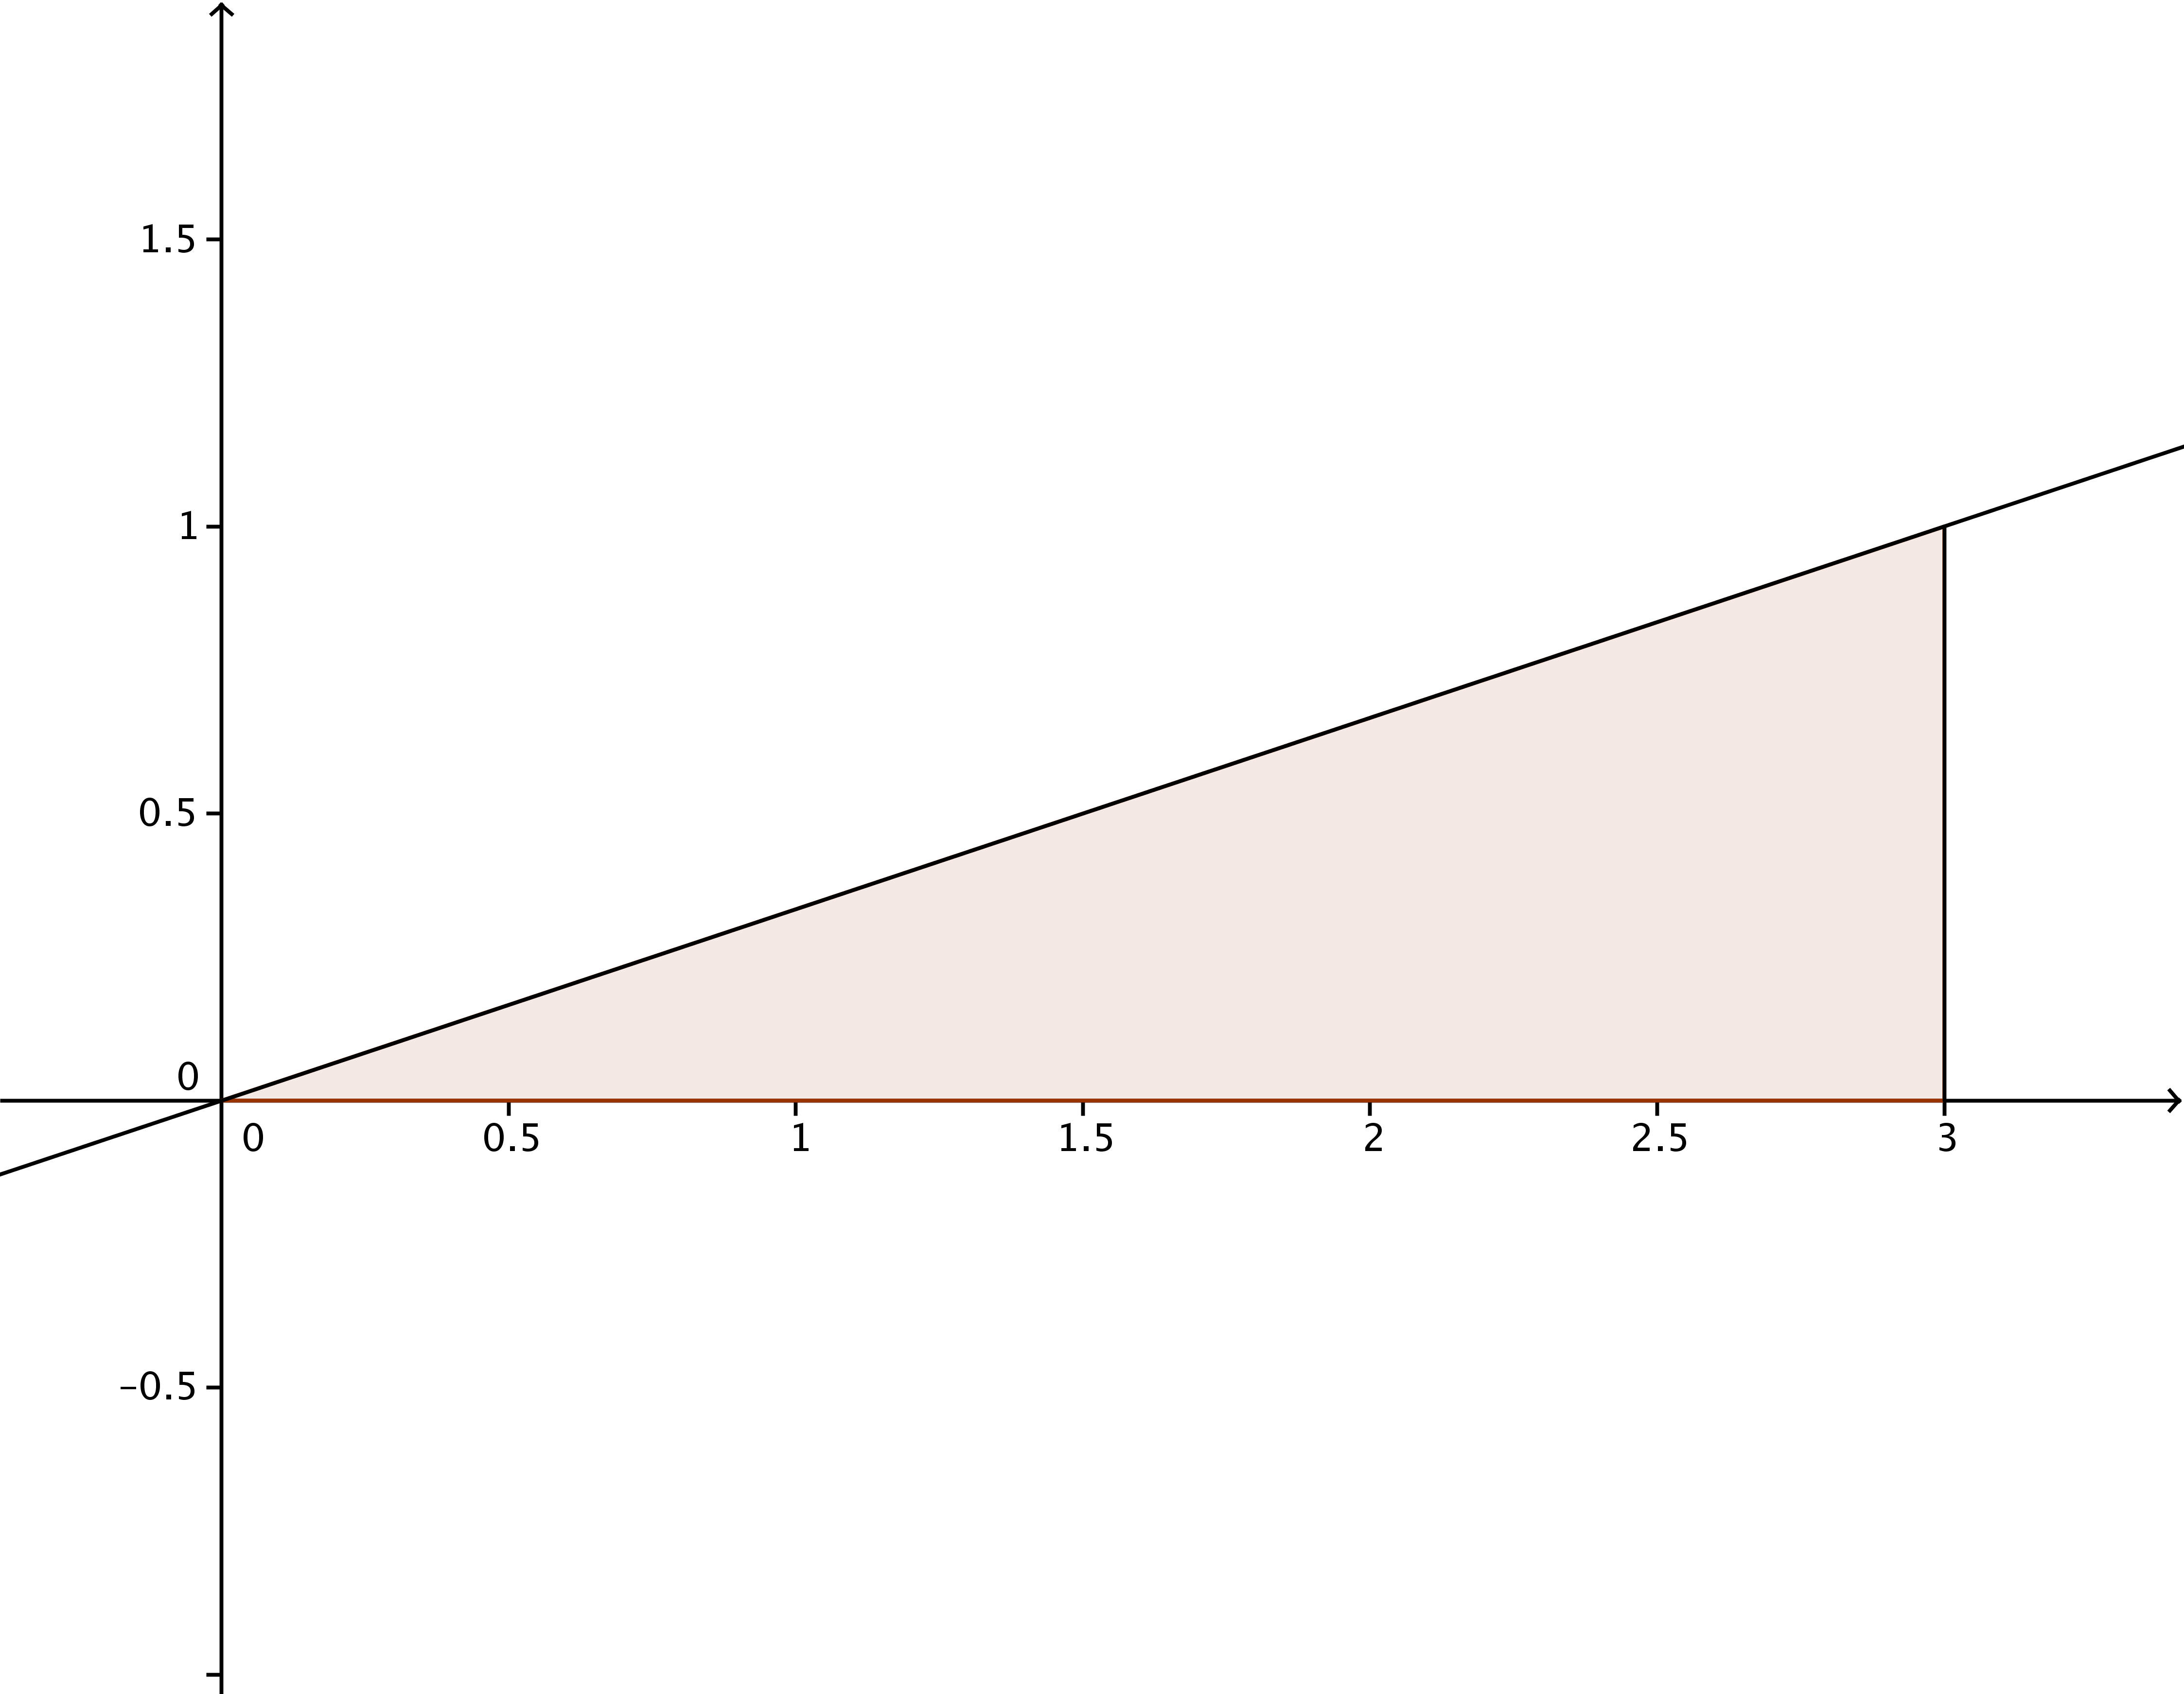
\includegraphics[width=3.5in]{Q11-4c.png} 
\end{center}

We're given the Type 2 region $0\leq y\leq 1$, $3y\leq x\leq 3$, but this is not very useful, since we don't have an antiderivative for $e^{x^2}$. Changing the order of integration, we can write $0\leq x\leq 3$, $0\leq y\leq \frac{1}{3}x$, giving us
\begin{align*}
 \int_0^1\int_{3y}^3 e^{x^2}\,dx\,dy & = \int_0^3\int_0^{x/3}e^{x^2}\,dy\,dx\\
& = \int_0^3 \frac{1}{3}xe^{x^2}\,dx\\
& = \left.\frac{1}{6}e^{x^2}\right|_0^3 = \frac{e^9-1}{6}.
\end{align*}

  \item $\di \int_0^1\int_{x^2}^1 x^3\sin(y^3)\,dy\,dx$

\begin{center}
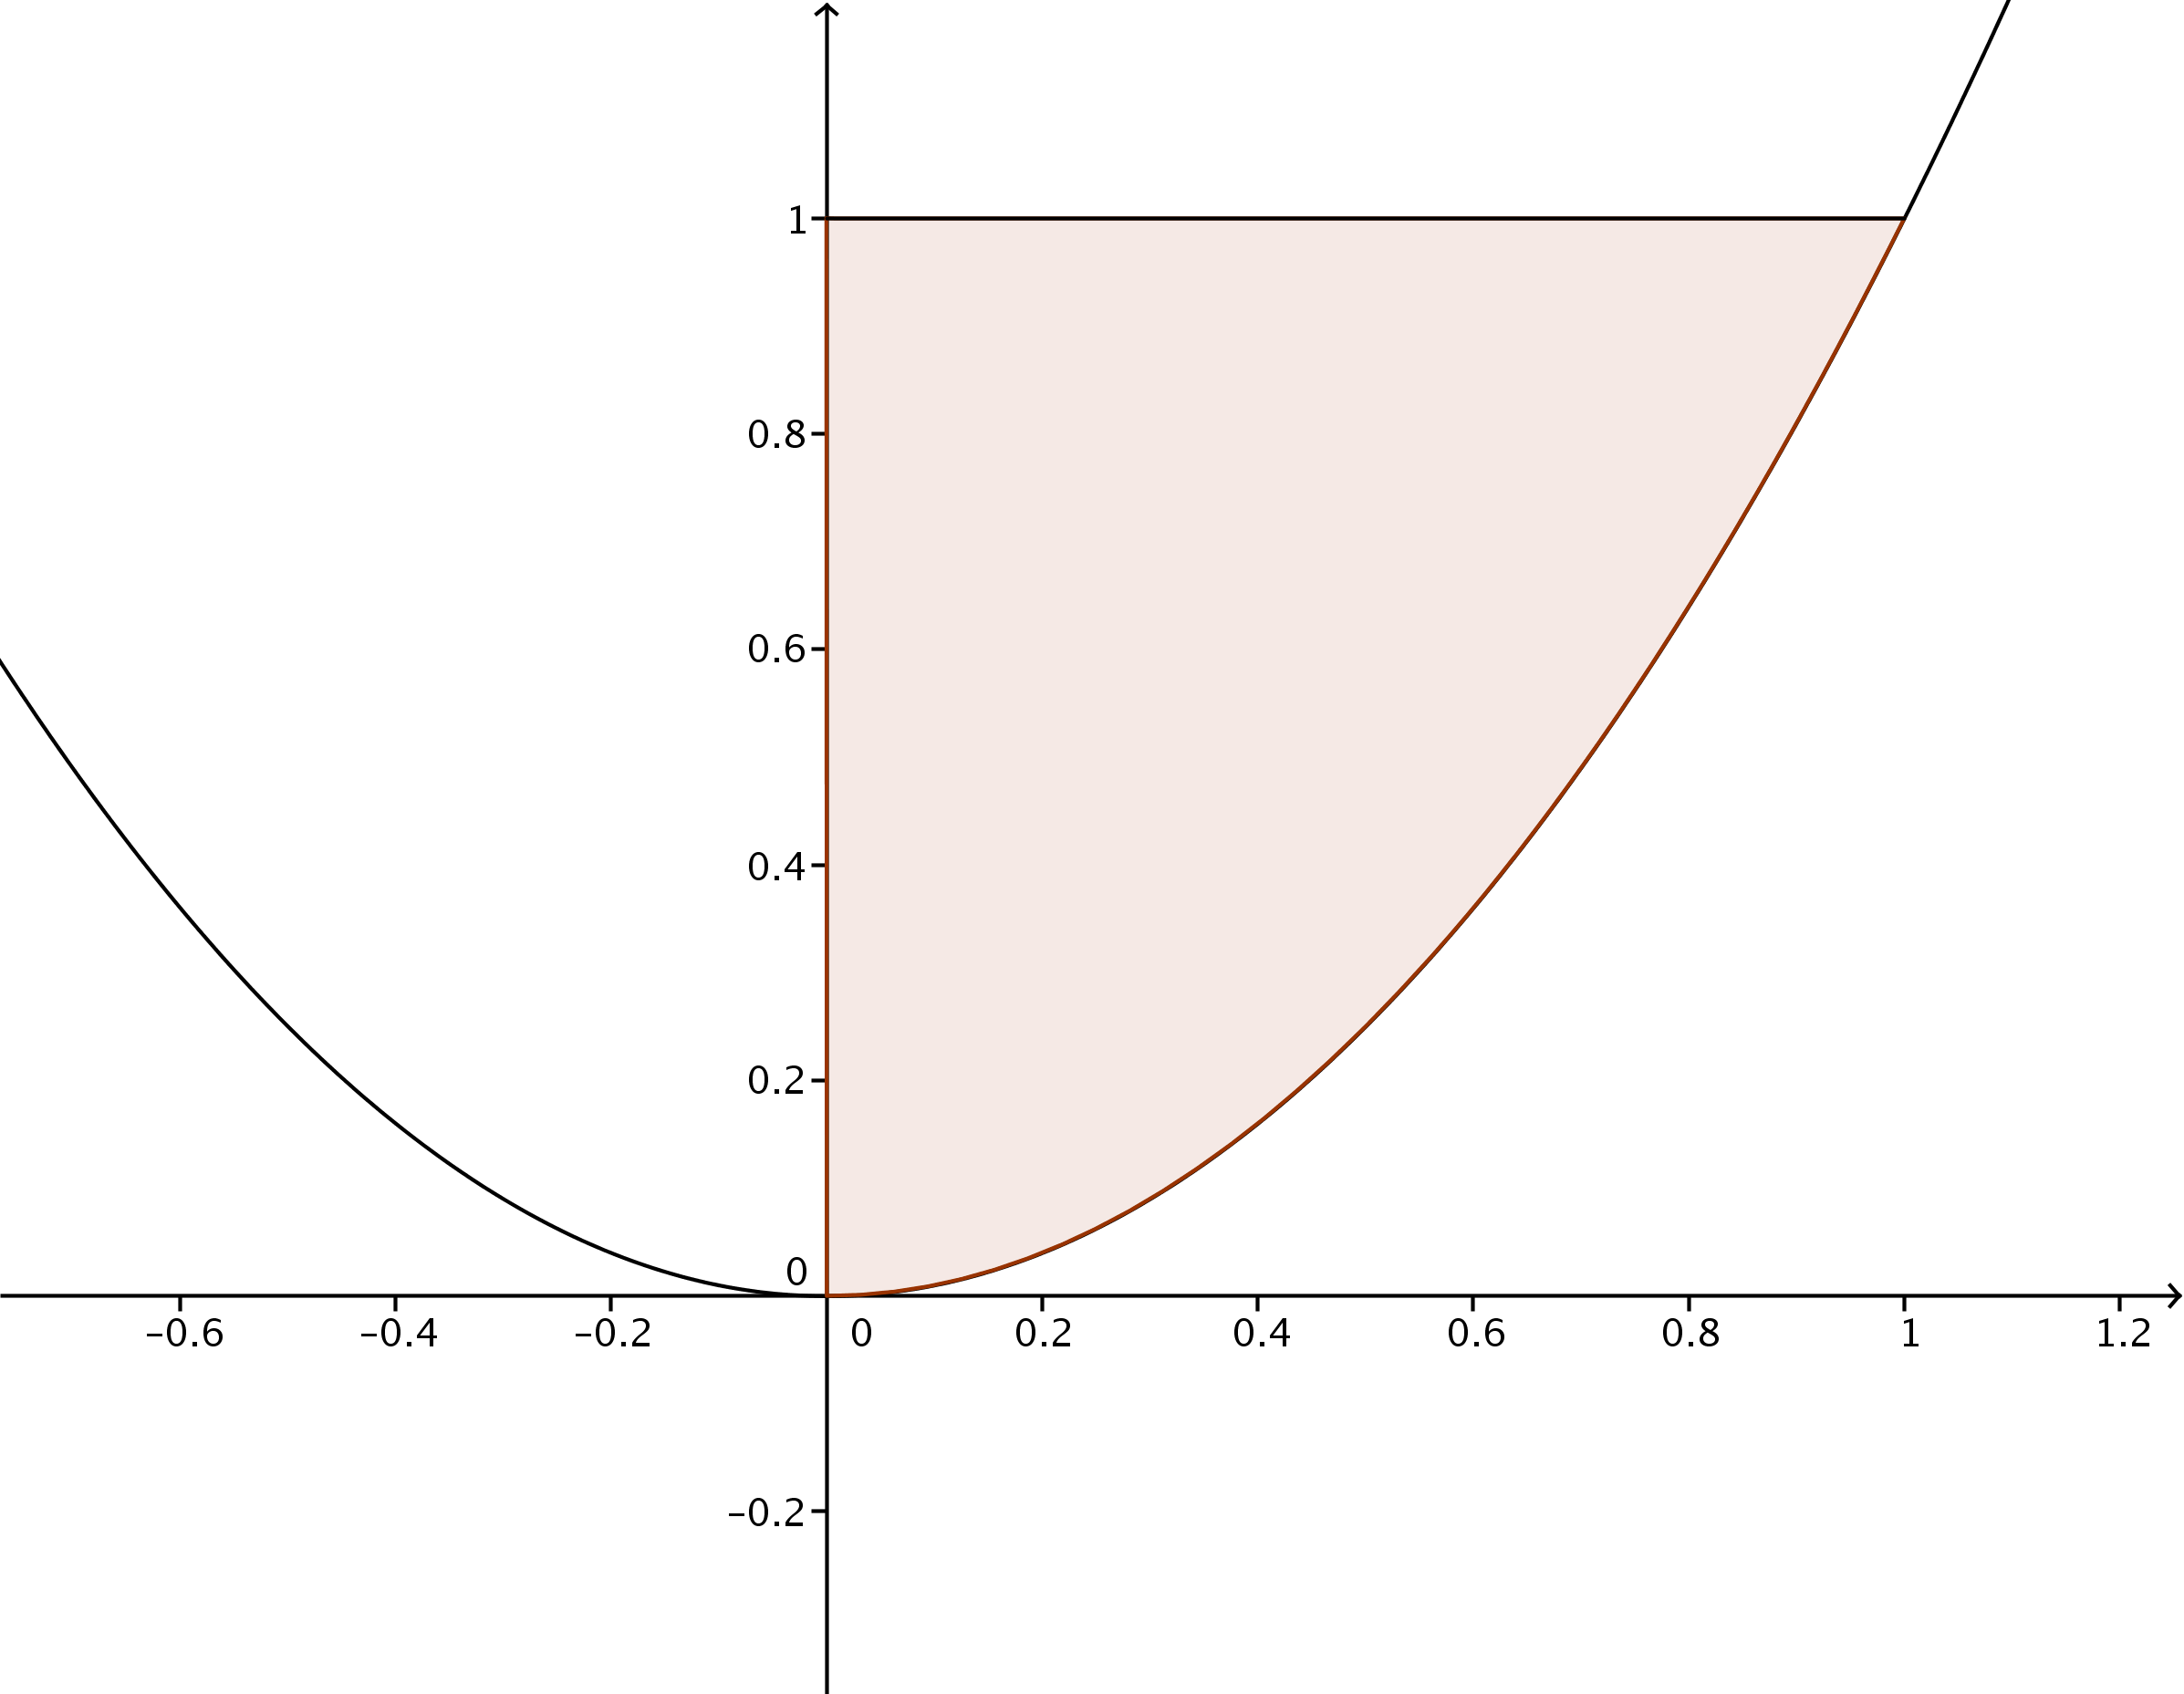
\includegraphics[width=3.5in]{Q11-4d.png} 
\end{center}

We're given the Type 1 region $0\leq x\leq 1$, $x^2\leq y\leq 1$. As a Type 2 region, it's given by $0\leq y\leq 1$, $0\leq x\leq \sqrt{y}$. Thus,
\begin{align*}
 \int_0^1\int_{x^2}^1 x^3\sin(y^3)\,dy\,dx & = \int_0^1\int_0^{\sqrt{y}}x^3\sin(y^3)\,dx\,dy\\
& = \int_0^1\left(\left. \frac{1}{4}x^4\sin(y^3)\right|_{x=0}^{x=\sqrt{y}}\right)\,dy\\
& = \int_0^1\frac{1}{4}y^2\sin(y^3)\,dy\\
& = \left.-\frac{1}{12}\cos(y^3)\right|_0^1\\
& = \frac{1-\cos(1)}{12}.
\end{align*}

 \end{enumerate}



 \end{enumerate}

\end{document}
 
